\section{Trace Funktion}\label{Validierung:Trace Funktion}
\label{section:ValidierungTraceFunktion}
Um die Trace Funktionalität in OpenPEARL zu prüfen werden die Umgebungsvariablen
werden wie folgt gesetzt:
\begin{itemize}
  \item \textbf{OpenPEARL\-\_LockTracer\-\_Enabled} = false
  \item \textbf{OpenPEARL\-\_LockTracer\-\_Path} = /tmp/LockTracer/
  \item \textbf{OpenPEARL\-\_LockTracer\-\_MaxEntries} = 1
\end{itemize}
Zum Testen wird die OpenPEARL Anwendung aus \cref{lst:OpenPEARLTraceTest}
verwendet. 
\begin{listing}[ht]
  \inputminted[frame=lines,linenos]{vim}{./OpenPEARL/TraceTest.prl}
  \caption{OpenPEARL Anwendung zum Testen der Trace Funktionalität}
  \label{lst:OpenPEARLTraceTest}   
\end{listing}
Es wird ein Thread \texttt{T1} erzeugt, welcher die \textit{SEMA} Variable
\texttt{test\_sema} insgesamt zehn Mal freigibt und in Besitz nimmt. Wird die
Anwendung ausgeführt wird keine Trace-Datei angelegt. Wird die Umgebungsvariable
\textbf{OpenPEARL\-\_LockTracer\-\_Enabled} auf \texttt{true} gesetzt, wird die
Trace-Datei aus \cref{lst:OpenPEARLTraceResult} erzeugt.
\begin{listing}[ht]
  \begin{minipage}[ht]{\linewidth}
    \begin{multicols}{2}
      \inputminted[linenos]{text}{./OpenPEARL/TraceTestResult.log}
    \end{multicols}
    \caption{Trace-Datei die bei aktivierter Trace Funktionalität aus \cref{lst:OpenPEARLTraceTest} erzeugt wird}
  \label{lst:OpenPEARLTraceResult}   
  \end{minipage}
\end{listing}

Die Tests zur Messung der Laufzeit und der Speicherauslastung werden in einer
virtuellen Debian 9 Linux Maschine mit 4 CPU Kernen und 2GB Arbeitsspeicher
durchgeführt. Das Host System läuft mit dem Betriebssystem macOS 10.15.4 und
verfügt über einen Intel Core i7 mit 3,1 GHz, 16GB Arbeitsspeicher und einer
512GB PCIe SSD. Zur Messung der Laufzeit wird das Pythonskipt aus
\cref{lst:Python_Benchmark_CPU} und zur Messung der Speicherauslastung das
Pythonskipt aus \cref{lst:Python_Benchmark_Memory} verwendet.
\begin{listing}[ht]
  \inputminted[frame=lines,linenos]{python}{./Python/benchmark_cpu.py}
  \caption{Pythonskipt zur Messung der Laufzeit}
  \label{lst:Python_Benchmark_CPU}   
\end{listing} 
\begin{listing}[ht]
  \inputminted[frame=lines,linenos]{python}{./Python/benchmark_memory.py}
  \caption{Pythonskipt zur Messung der Speicherauslastung}
  \label{lst:Python_Benchmark_Memory}   
\end{listing}
Für die Tests wird eine OpenPEARL Anwendung verwendet, welche 10 Threads
erzeugt, welche jeweils nacheinander zwei \textit{SEMA} Objekte in Besitz nehmen
und wieder freigeben. Dabei verwendet der Thread \textit{T1} die Objekte
\textit{L01} und \textit{L02}, der Thread \textit{T2} die Objekte \textit{L02}
und \textit{L03}, bis zum letzten Thread \textit{T10}, welcher die Objekte
\textit{L10} und \textit{L01} verwendet. Ingesamt werden 400.000 Einträge
erzeugt. Das Ergebnis der Laufzeitmessung ist in \cref{fig:BenchmarkCpuResults}
dargestellt. 
\begin{figure}[ht]
  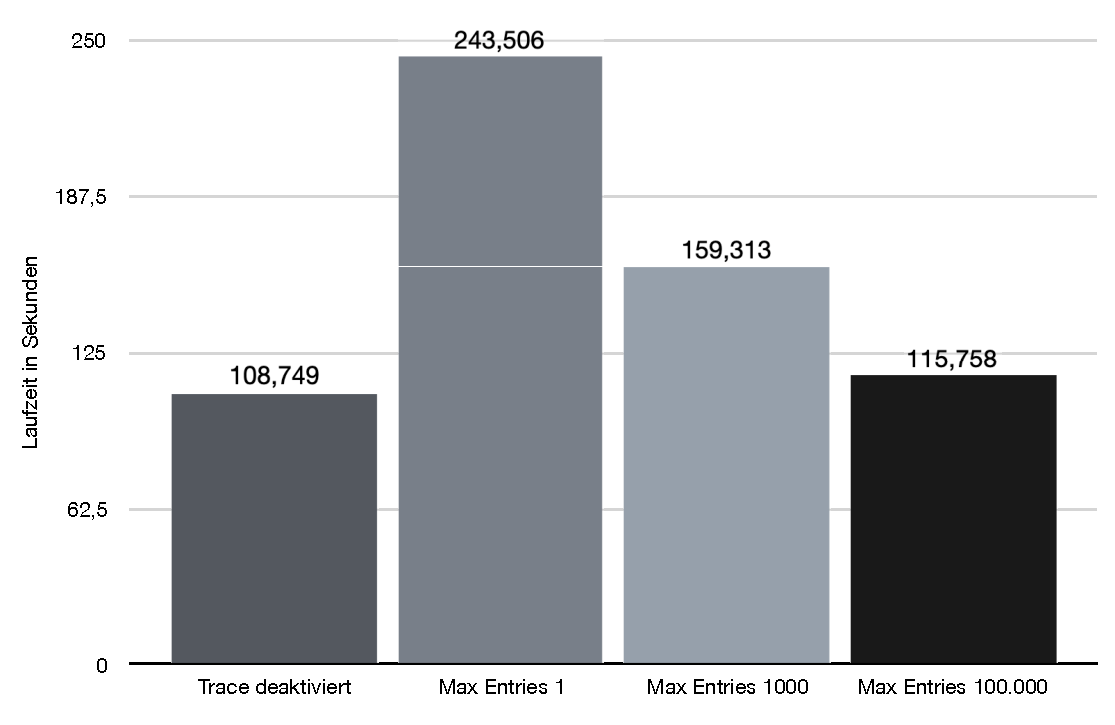
\includegraphics[width=\linewidth]{Benchmark_CPU_Results.eps}
  \caption{Ergebnisse der Laufzeitmessung der Trace-Funktionalität in OpenPEARL}
  \label{fig:BenchmarkCpuResults}
\end{figure}
Eine höhere Anzahl an gepufferten Objekten führt bis zu einem bestimmten Punkt
zu einer besseren Laufzeit. Bei einer Puffergröße von 100.000 gibt es nur noch
einen sehr geringen Unterschied zwischen aktivierter und deaktivierter
Trace-Funktionalität. Wird die Puffergröße auf 500.000 gesetzt, passen alle
Einträge in den Puffer und werden beim Beenden der Anwendung in die Trace-Datei
geschrieben. Die Laufzeit verbessert sich bei dieser Größe jedoch nicht weiter,
sondern verschlechtert sich leicht. Bereits der Unterschied zwischen den
Puffergrößen 1.000 und 100.000 zeigt, dass die Puffergröße nicht beliebig hoch
gesetzt werden sollte, um eine optimale Laufzeit zu erhalten. Die Puffergröße
muss individuell für das Zielsystem ermittelt werden. Das Ergebnis der Messung
der Speicherauslastung ist in \cref{fig:BenchmarkMemoryResults} dargestellt.
\begin{figure}[ht]
  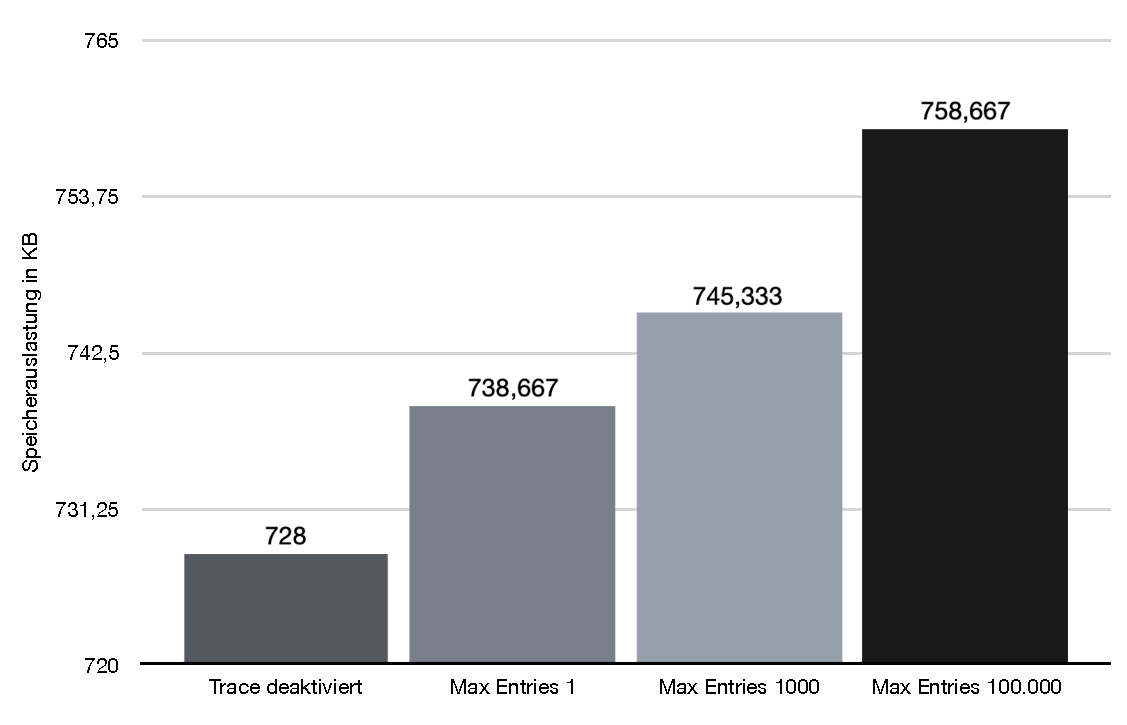
\includegraphics[width=\linewidth]{Benchmark_Memory_Results.eps}
  \caption{Ergebnisse der Speicherauslastung der Trace-Funktionalität in OpenPEARL}
  \label{fig:BenchmarkMemoryResults}
\end{figure}
Je größer der verwendete Puffer ist, desto höher ist auch die
Speicherauslastung. Für das verwendete Testsystem ist eine Puffergröße von 1.000
ein guter Kompromiss zwischen Laufzeit und Speicherauslastung. Ist die Laufzeit
wichtiger und die Speicherauslastung kein Problem, sollte eine Puffergröße von
100.000 gewählt werden.

\section{Analyse Programm}
\label{section:ValidierungAnalyseProgramm}
Für die chronologische Darstellung der Lockobjekte wird die Trace-Datei aus
\cref{lst:ExampleTraceFile} mit drei Threads und neun Lockobjekten.
\begin{listing}[ht]
  \begin{minipage}[ht]{\linewidth}
    \begin{multicols}{3}
      \inputminted[linenos]{text}{./Examples/ExampleTraceFile.log}
    \end{multicols}
    \caption{Beispielhafte Trace-Datei mit einem potenziellen Deadlock}
    \label{lst:ExampleTraceFile}
  \end{minipage}
\end{listing}
In dem Beispiel gibt es zusätzlich zwei Einträge mit dem gleichen Zeitstempel in
den Zeilen 3 und 4 sowie in den Zeilen 13 und 14. Die Ausgabe der Anwendung aus
\cref{section:Implementierung:Analyse Programm} ist in
\cref{fig:LockTraceVisualization} dargestellt.
\begin{figure}[ht]
  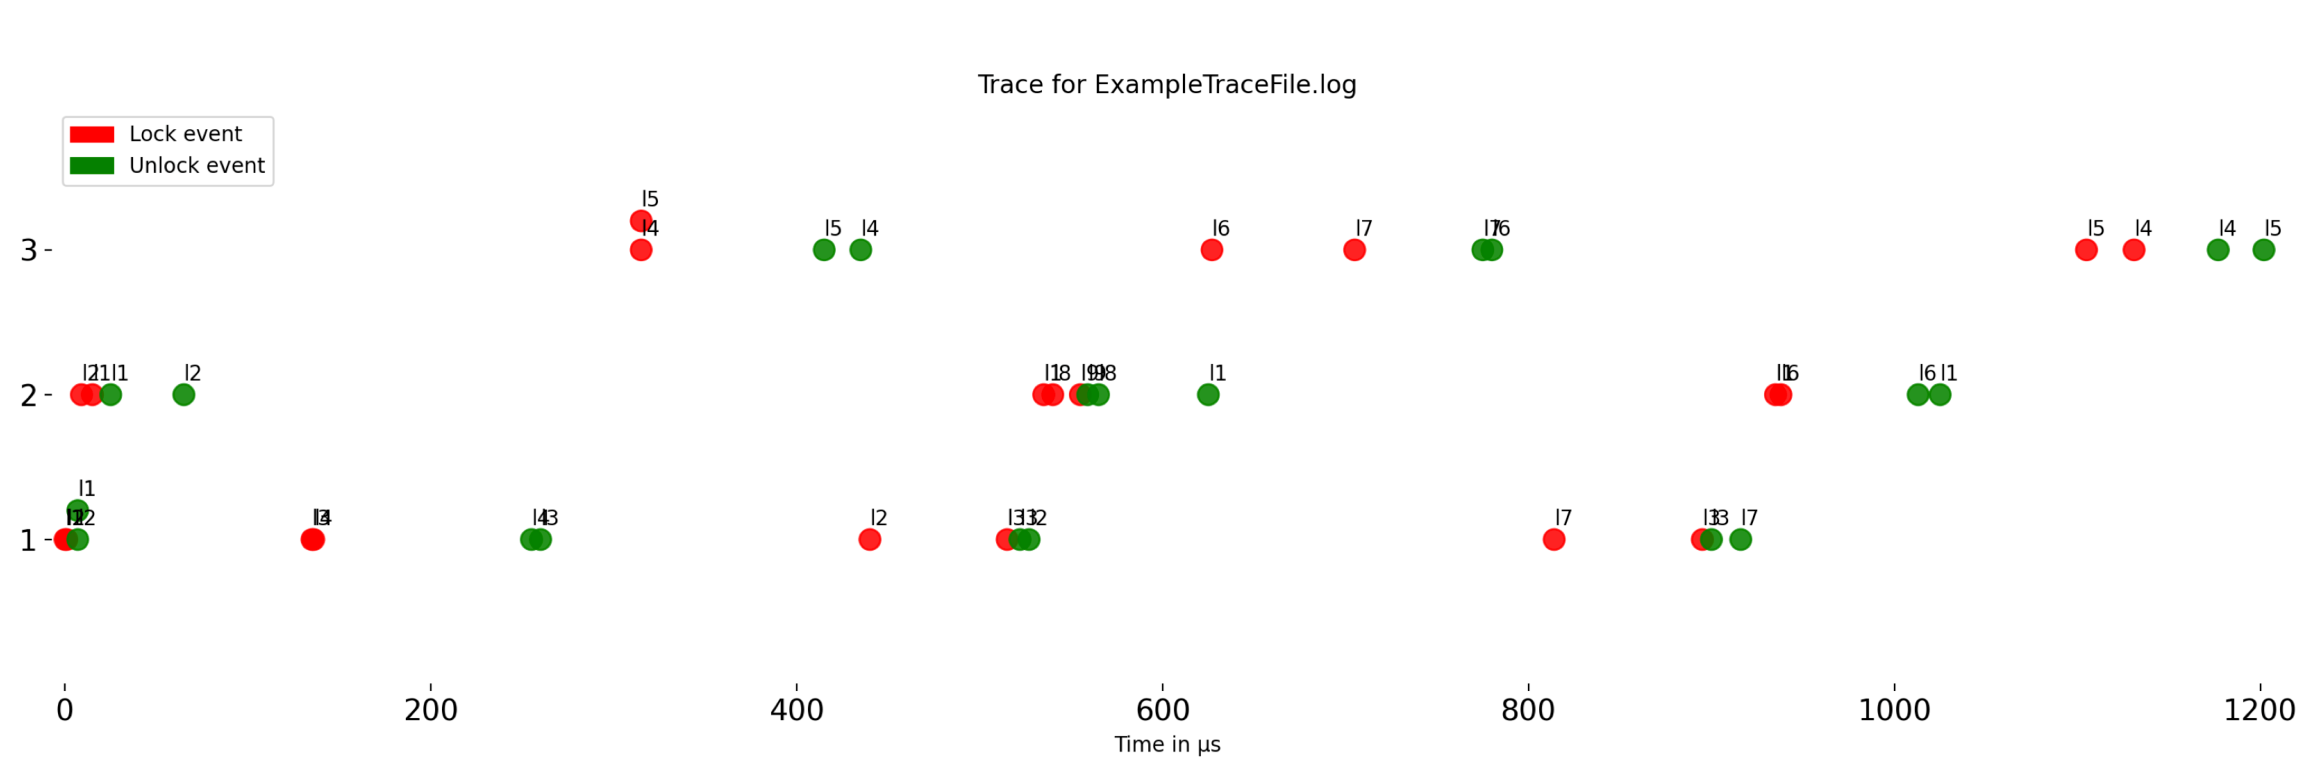
\includegraphics[width=\linewidth]{ExampleTraceFile.eps}
  \caption{Ausgabe der Analyse-Anwendung}
  \label{fig:LockTraceVisualization}
\end{figure}
Die überlappenden Logeinträge können auseinander gezogen werden in dem in den
Graphen hineingezoomt wird. Wird zum Beispiel auf die ersten 70 Mikrosekunden
vergrößert, werden die Logeinträge auseinander gezogen siehe
\cref{fig:LockTraceVisualizationZoomed}.
\begin{figure}[ht]
  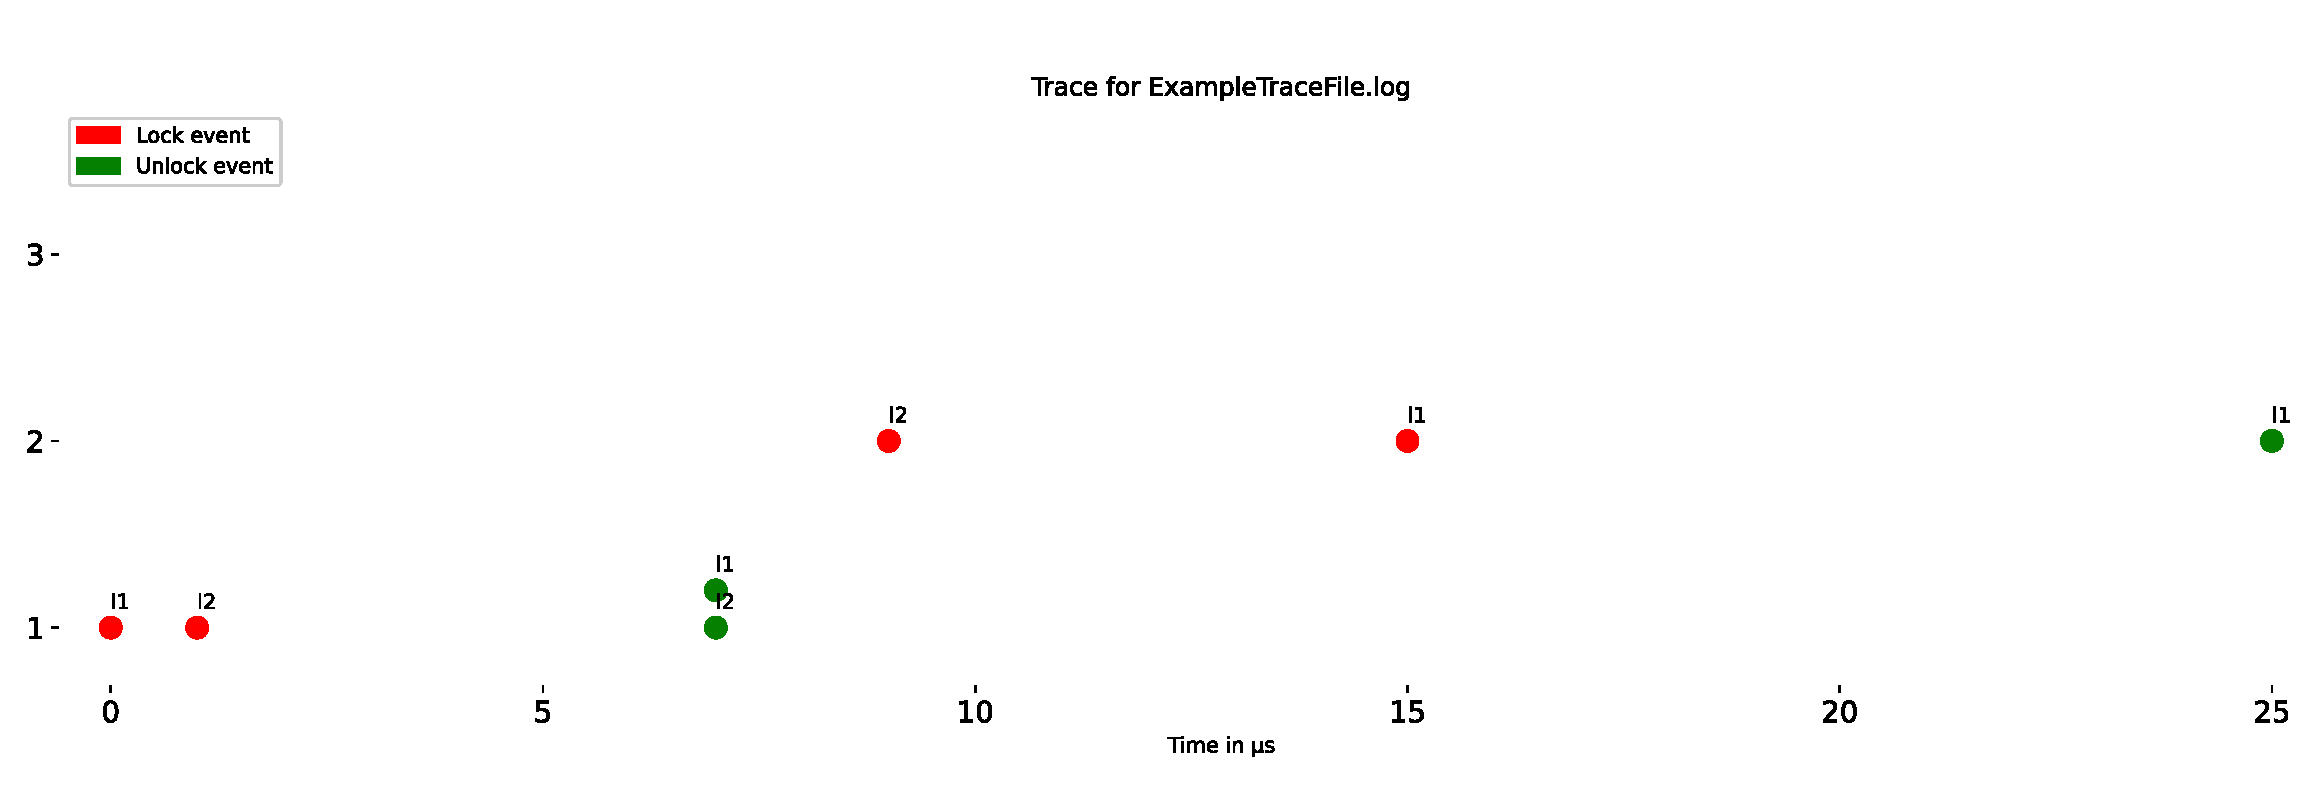
\includegraphics[width=\linewidth]{ExampleTraceFileZoomed.eps}
  \caption{Vergrößerte Darstellung von \cref{fig:LockTraceVisualization}}
  \label{fig:LockTraceVisualizationZoomed}
\end{figure}
Die beiden Logeinträge mit den gleichen Zeitstempel sind bei 7 Mikrosekunden
korrekt vertikal versetzt dargestellt.

\section{Visualisierung von potenziellen Deadlocks}
\label{section:DeadlockVisualization}
Für die Visualisierung von potenziellen Deadlocks wird wieder die Trace-Datei
aus \cref{lst:ExampleTraceFile} verwendet. In dem Beispiel gibt es genau einen
potenziellen Deadlock zwischen den Threads \textit{1} und \textit{2}. In den
Zeilen 1 und 2 nimmt der Thread \textit{1} die Lockobjekten \textit{l1} und
\textit{l2} nacheinander in Besitz. In den Zeilen 5 und 6 nimmt der Thread
\textit{2} die Lockobjekte \textit{l2} und \textit{l1} nacheinander in Besitz.
Der potenzielle Deadlock entsteht, da der Thread \textit{1} zuerst das
Lockobjekt \textit{l1} in Besitz nehmen kann und bevor dieser das Lockobjekt
\textit{l2} in Besitz nehmen kann, kann der Thread \textit{2} das Lockobjekt
\textit{l2} bereits in seinen Besitz genommen haben. Dadurch blockieren sich
beide Threads gegenseitig und ein Deadlock entsteht. Die Ausgabe der Anwendung
zur Erkennung und Visualisierung von potenziellen Deadlocks ist in
\cref{fig:DeadlockVisualization} dargestellt.
\begin{figure}[ht]
  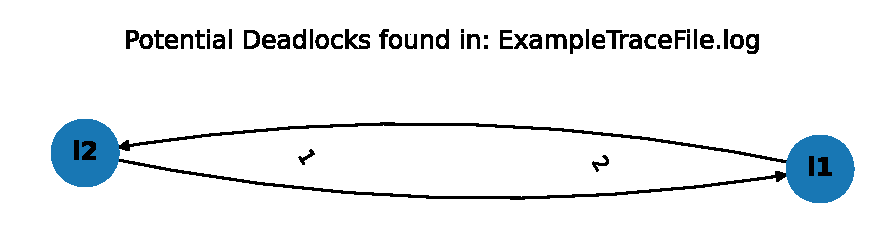
\includegraphics[width=\linewidth]{ExamplePotentialDeadlocks.eps}
  \caption{Ergebnis der Erkennung von potenziellen Deadlocks aus \cref{lst:ExampleTraceFile}}
  \label{fig:DeadlockVisualization}
\end{figure}
Die Beschriftung der Kanten erfolgt immer zum Ende der Kante hin, zum Beispiel
gehört die Beschriftung \textit{1} zu der Kante von \textit{l1} zu \textit{l2}.
Zusätzlich zur grafischen Darstellung werden die Ergebnisse als
Zyklische-Lock-Dependency-Chain auf der Konsole ausgegeben. Für die verwendete
Trace-Datei wird "(1,l2,{l1}) (2,l1,{l2})" als potenzieller Deadlock auf der
Konsole ausgegeben.